% -*-coding: utf-8;-*-
%%%%%%%%%%%%%%%%%%%%%%%%%%%%%%%%%%%%%%%%%%%%%%%%%%%%%%%%%%%%%%%%%
% Глава 2 - Замена линейного регулятора на нейросетевой

Подходы линейной теории автоматического регулирования широко
применяются на практике в самых различных областях.  Во многих случаях
использование линейных регуляторов и линейных моделей объектов
управления позволяет достичь необходимого качества систем управления.
Однако по мере совершенствования науки и техники, всё более актуальным
становятся задачи нелинейного управления.  В частности, это связано
как с повышением требований к качеству управления, когда учет
нелинейных свойств выходит на первый план, так и с рассмотрением новых
задач, решение которых с помощью линейной теории управления
оказывается невозможным.  Искусственные нейронные сети являются одним
из современных подходов, позволяющих реализовать нелинейное управление
в технических системах.

% О достоинствах (в 1-й главе):
% - неаналитичность решения
% - теоретически неограниченная мощность
% - нетребовательность к ресурсам (в режиме работы, а не обучения)
% - и пр.

Представляется актуальным разработать методические рекомендации по
замене линейного регулятора на нейросетевой, рассмотрев задачу выбора
архитектуры нейросети, а также выявить факторы, влияющие на качество
имитации исходного регулятора.

%TODO
%Следует также систематически сравнить
%нейросетевой регулятор с исходным линейным и выяснить их взаимные
%особенности.

Перечисленные вопросы слабо освещаются в публикациях.  В то же время,
их важность трудно оспорить --- применение любой альтернативной
парадигмы (и нейронных сетей в том числе) без понимания её свойств и
разработанной методической базы представляется ненаучным и чреватым
неожиданными проблемами в инженерной практике.

\section{Постановка задачи}

Рассмотрим систему автоматического регулирования (САР) с обратной
связью, изображенную на \figref{fig:ctrlloop}.  Будем считать, что
состояние объекта непосредственно измеряется на выходе, однако в
канале наблюдения присутствует аддитивная помеха $n(t)$ с некоторыми
постоянными свойствами.  Параметры объекта управления также постоянны
во времени.  В системе имеется линейный регулятор, поддерживающий
состояние объекта близким к заданной траектории $r(t)$.

\begin{figure}[h]
  \centering
  \input{rawctrlloop.eps_t}
  \caption{Исходная система управления.}
  \label{fig:ctrlloop}
\end{figure}

Решим задачу синтеза нейросетевого регулятора (НС--Р) для замены
имеющегося в описанной системе.  В качестве примера исходного возьмем
ПИД регулятор как наиболее типичный и распространенный в промышленных
системах автоматического регулирования.  Считая, что исходный
регулятор обеспечивает устойчивость и некоторое удовлетворительное
качество управления, можно ожидать, что достаточно точный имитатор
будет управлять системой подобно.  Качество обучения искусственной
нейронной сети определяется выбором архитектуры, обучающих данных и
параметров методики обучения.  Исследуем влияние перечисленных
факторов в задаче имитации исходного регулятора.

Будем рассматривать систему управления и её составные части в
дискретном времени с постоянным шагом дискретизации, достаточно малым,
чтобы охватить всю значимую для данной системы полосу частот.  Данный
подход позволяет моделировать саму САР и нейронные сети на компьютере.

% Архитектура НС-Р (структура входов, количество нейронов)
% Обучающая выборка (критерий достаточности объема, влияние вида выборки на качество обучения)
%TODO
% Сравнение НС-Р и ПИД (статическая ошибка, быстродействие, частотная характеристика)

%\section{Методика синтеза}???

Представим действие исходного линейного регулятора с
\figref{fig:ctrlloop} по управлению объектом как функцию $f(.)$:
\begin{equation}\label{eq:raw_controller}
  u_k=f(e_k,\mathbf{s})
\end{equation}

\noindent где $\mathbf{s}$ --- внутреннее состояние регулятора
(``память''), изменяющееся каждый такт времени по некоторому правилу.
Нейросетевой регулятор $\NN^p(.)$ должен обеспечить имитацию $f(.)$
физически реализуемым способом.  Используя квадратичный критерий,
задача синтеза НС--Р представляется в виде:
\begin{equation}\label{eq:nnp_synthesis_task}
  \sum\limits_k\big(f(e_k,\mathbf{s})-\NN^p(\mathbf{i}_k)\big)^2
  \rightarrow\min\limits_{\mathbf{i}_k\in\mathbf{I}}
\end{equation}

\noindent где $\mathbf{i_k}$ --- некоторая информация, доступная о
системе управления к моменту времени $t_k$, в том числе, ошибка
управления $e_k$, что определяет условие физической реализуемости.
$\mathbf{I}$ --- это область возможных значений $\mathbf{i_k}$ для
регулятора.  Способ формирования вектора $\mathbf{i}_k$, необходимого
для имитации исходного регулятора нейронной сетью, является отдельной
задачей, которую необходимо решить.

Сформулированная задача эквивалентна общей задаче нейросетевой
аппроксимации неизвестной фунции $f(.)$, заданной таблично
(см.~\eqref{eq:supervised_learning_task}) с помощью нейронной сети
$\NN(.)$.  А.~Н. Колмогоров в теореме о представлении непрерывных
функций нескольких переменных~\cite{kolmog57}, доказал существование
такой функции.  В работе \cite{rumelhart86} был предложено обобщенное
дельта-правило ({\em generalized delta-rule}) для обратного
распространения ошибки в многослойном персептроне, дающее
конструктивную основу для поиска решения.

Таким образом, задача синтеза НС--Р может быть подразделена на
следующие решаемые последовательно подзадачи:
\begin{enumerate}
\item Выбор архитектуры НС--Р, в том числе, вектора информации о
  системе $\mathbf{i}_k$.
\item Сбор обучающих данных.
\item Собственно обучение НС--Р.
\item Проверка качества имитации и функционирования НС--Р.
\end{enumerate}

Рассмотрим перечисленные подзадачи, делая упор на методологию их
решения, обоснование выбора среди альтернативных вариантов и
специальные случаи.  В сумме предлагаемые подходы обеспечивают
методический базис для синтеза нейросетевого регулятора в качестве
замены линейного.

%Третья подзадача решается общеизвестным способом
%(см. п.~\ref{nn_learning_algorithms}).  Рассмотрим первые две
%подзадачи.

%\section{Методические рекомендации по синтезу нейросетевого регулятора}
%{\LARGE N/A}

\section{Архитектура нейросетевого регулятора}\label{nnc_arch}

ПИД регулятор представляет собой динамическую систему, обладающую
памятью (кроме простейшего случая пропорционального управления).  Для
адекватной имитации нейронная сеть регулятора также должна обладать
динамическими свойствами.  При синтезе нейросетевой модели объекта
управления (см. п.~\ref{identif_and_nnp}), эта задача решается либо за
счет добавления обратных связей, либо за счет организации внешней
памяти в виде элементов задержки.

Сравнивая задачу обучения НС--Р с задачей синтеза нейросетевой модели
объекта следует при очевидном сходстве (имитация некоторой линейной
системы) отметить два фундаментальный различия.  Во-первых, НС--О
может быть реализована как в виде автономной модели поведения, так и в
виде зависимой от объекта модели предсказания, в то время как НС--Р
должен полностью заменить исходный регулятор.  Во-вторых, назначение
НС--О --- копирование поведения объекта управления, а НС--Р должен
быть сначала обучен подобно исходному линейному регулятору, но потом,
в соответствии с заданными правилами (например, минимизация
среднеквадратической ошибки или подстройка под нестационарный объект),
может изменить свои свойства.  Буквальное повторение свойств исходного
линейного регулятора не является самоцелью, а лишь позволяет
сопоставить нейросетевой и традиционный линейный регуляторы.  По этой
причине не имеет смысла формировать архитектуру нейросетевого
регулятора базируясь на свойстве линейности исходного.

Как и в случае с синтезом НС--О возникает задача выбора между
статической и динамической (с обратными связями) архитектурами
нейронной сети.  Аргументом в пользу динамической нейронной сети
является наиболее очевидный путь имитации свойств линейной
динамической системы с помощью автономной модели, а также более общий
характер решения задачи.  Вместе с тем, у динамической нейронной сети
имеются как недостатки общего плана, упомянутые в
п.~\ref{identif_and_nnp}, так и специфические, проявляющиеся при
использовании обратных связей в НС--Р:

\begin{enumerate}
\item эффект исчезающего градиента при обучении по методу BPTT;
\item увеличение требований к ресурсам и усложнение алгоритма обучения
      в контуре, вызванное процедурой обращения времени;
\item усложнение анализа устойчивости системы за счет появления еще
      одного контура обратной связи с нелинейным элементом (нейросетью).
\end{enumerate}

Применение статической нейронной сети для реализации НС--Р не имеет
перечисленных недостатков, кроме того, обучение статической нейросети
в целом осуществляется быстрее, чем динамической.  Однако, как и в
случае с нейросетевой моделью объекта управления, следует с помощью
надлежащего формирования структуры входов нейросети обеспечить
динамические свойства НС--Р, аналогичные имеющимся у ПИД регулятора в
контуре. 

%\subsection{Структура входов нейросети}
\label{nnc_inputs}%
Рассмотрим несколько вариантов формирования вектора входных значений
$\mathbf{i}_k$ для НС--Р (см. \eqref{eq:nnp_synthesis_task}).
Обязательно следует проверить вариант подключения, аналогичный
исходному регулятору.  В этом случае на вход подается только значение
ошибки в текущий момент времени $e_k$.  Как было показано ранее при
построении нейросетевой модели объекта, этот вариант подключения
статической нейронной сети не может обеспечить адекватную имитацию
свойств динамической системы.  Чтобы преодолеть ограничение
статического отображения надо искусственно организовать память с
помощью повторения прошлых входов $e_k\ldots e_{k-d}$.  Поэтому
исследуем поведение НС--Р при различных значениях емкости памяти:
$0\le d\le 4$.

Рассмотрим также варианты подключения НС--Р с входами $e_k,\Delta e_k$
и $r_k,e_k$.  Первый вариант обеспечивает нейросеть информацией о
динамике с помощью дискретной производной сигнала ошибки управления, а
второй представляет собой объединение концепций управления по
возмущению $r(t)$ и отклонению $e(t)$.

Для сравнения перечисленных вариантов формирования входного вектора
НС--Р была проведена серия экспериментов.  Ниже приводится постановка
и результаты одного из них.

% nn/dpid.new/contrp/...
Эксперимент проводился в условиях стохастической уставки при наличии
случайной аддитивной помехи в наблюдаемом выходе объекта управления.
Формирующие фильтры уставки $R^*(z)=\frac{0.625z}{z-0.779}$ и помехи
$N^*(z)=0.4$.  Объект $P^*(z)=\frac{z}{z-0.5}$ управлялся ПИД
регулятором $C^*(z)=0.4 + 0.5\frac{z}{z-1} +
0.05\frac{z^2-2z+1}{z(z-1)}$.  Регулятор был настроен на ступенчатом
возмущающем сигнале по критерию минимизации длительности переходного
процесса при максимальном перерегулировании в пределах 4\% амплитуды
возмущающего сигнала.

Нейронная сеть регулятора имела архитектуру $\NN^p_{x,7,3,1}$,
где $x$ --- размерность входного вектора.  Обучение осуществлялось на
выборке длиной 200 в течение 400 эпох, а контрольная выборка имела
длину 500, причем если ошибка на контрольной выборке начинала
возрастать, то обучение досрочно прекращалось.  Критерием обучения
являлась минимизация среднеквадратичной ошибки воспроизведения.

\begin{table}[ht]
\centering
\caption{Сравнение точности имитации ПИД регулятора вне контура управления
         при различном способе формирования входного вектора НС--Р и
         различных параметрах уставки и помехи (см. также
         \figref{fig:pretr_input_vec_rus})}
\label{tabl:nnc_pretr_input_vec}
\begin{tabular}{|c|l|c|c|c|c|}
\hline
\multicolumn{2}{|r|}{Эксперимент} & {\sf А} & {\sf Б} & {\sf В} & {\sf Г}\\
\hline
\multicolumn{2}{|r|}{Уставка} &
  \multicolumn{2}{|c|}{Стохастическая $R^*(z)$} & $\sin(t)$ & $0$ \\
\hline
\multicolumn{2}{|r|}{Помеха} & $N^*(z)=0.4$ & $N^*(z)=0.7$ & $N^*(z)=0.4$ & $N^*(z)=0.4$\\
\hline\hline
N   & Входной               & \multicolumn{4}{|c|}{Среднеквадратическая ошибка} \\
пп. & вектор $\mathbf{i}_k$ & \multicolumn{4}{|c|}{на контрольной выборке}\\
\hline
1 & $e_k$                 & 0.3228 & 0.2906 & 0.1299 & 0.0027\\
2 & $e_k,e_{k-1}$         & 0.2993 & 0.2710 & 0.1291 & 0.0022\\
3 & $e_k\ldots e_{k-2}$   & 0.2709 & 0.2459 & 0.1270 & 0.0016\\
4 & $e_k\ldots e_{k-3}$   & 0.2482 & 0.2284 & 0.1240 & 0.0013\\
5 & $e_k\ldots e_{k-4}$   & 0.2385 & 0.2163 & 0.1188 & 0.0013\\
6 & $e_k,\Delta e_k$      & 0.2980 & 0.2738 & 0.1293 & 0.0023\\
7 & $r_k,e_k$             & 0.0388 & 0.0968 & 0.0039 & 0.0040\\
\hline
\end{tabular}
\end{table}

\begin{figure}[h]
\centering
\includegraphics[width=0.8\textwidth,%
  height=0.35\textheight]{pretr_input_vec_rus}
\caption{Среднеквдратическая ошибка управления в случае разных
  пробных сигналов и входных векторов НС--Р.}
\label{fig:pretr_input_vec_rus}
\end{figure}

В \tablref{tabl:nnc_pretr_input_vec} результаты эксперимента приведены
в столбце {\sf А}.  Анализ значений среднеквадратичной ошибки
показывает, что увеличение емкости памяти прошлых входов позволяет
лишь незначительно уменьшить ошибку имитации (строки таблицы 1--5).
Вариант с ошибкой и её первой разностью $e_k,\Delta e_k$ (строка 6)
показывает близкие результаты с вариантом $e_k,e_{k-1}$ (строка 2).
Очевидно, что для НС--Р эти варианты информационно эквивалентны.
Наилучшее качество имитации исходного регулятора было достигнуто НС--Р
с входным вектором $r_k,e_k$, причем достигнутый уровень ошибки в этом
случае оказался меньше почти на порядок, чем в остальных.

Эксперименты показали, что при увеличении мощности помехи
относительное преимущество НС--Р с входным вектором $r_k,e_k$
уменьшается (столбец {\sf Б} таблицы).  Таким образом, применение в
качестве входного вектора $e_k\ldots e_{k-d}$ может оказаться в
некоторых случаях оправданным.

Были также рассмотрены случаи предварительного обучения НС--Р по
детерминированной уставке различной формы.  По результатам
экспериментов наилучшим вариантом формирования входного вектора с
большим отрывом оказалось совмещенное управление по возмущению и
отклонению: $r_k,e_k$ (строка 6).  Оказалось также, что результирующий
уровень ошибки при периодической уставке практически не зависит от ее
формы.  В частности, числовые значения среднеквадратичной ошибки на
гармоническом сигнале (столбец {\sf В}
\tablref{tabl:nnc_pretr_input_vec}) и на меандре примерно одинаковы.

Отдельно был рассмотрен случай задачи стабилизации, когда уставка
постоянна, например, равна 0 (столбец {\sf Г}
\tablref{tabl:nnc_pretr_input_vec}).  Нейросетевой регулятор с
входным вектором $r_k,e_k$ показал худший результат, чем любой из
вариантов с повторением прошлых значений ошибки.  Видно, что
отсутствие влияния уставки на нейронную сеть в данном случае делает
наличие входа $r_k$ не только бесполезным, но и вредным.

Проводились также эксперименты с объектом управления с чистым
запаздыванием и объектом управления второго порядка, анализ которых
обнаружил те же закономерности.

По результатам проведенных экспериментов можно сформулировать
некоторые рекомендации по формированию входного вектора нейросетевого
регулятора по критерию наилучшей имитации исходного ПИД регулятора:

\begin{itemize}\label{nnc-inputs-rules}
\item
В случае задачи стабилизации (постоянное значение уставки)
рекомендуется использовать входной вектор с ошибкой и её первой
разностью $e_k,\Delta e_k$ или один из вариантов с повторением прошлых
значений: $e_k\ldots e_{k-d}$.  При увеличении емкости памяти прошлых
значений (параметр $d$) качество имитации при наличии помехи будет
возрастать.

\item
В случае изменяющегося значения уставки предпочтительным является
совмещенное управление по возмущению и отклонению: $r_k,e_k$.  При
значительном уровне помехи улучшить качество имитации можно вводя и
увеличивая память прошлых состояний.  Входной вектор в этом случае
будет иметь вид $r_k,e_k\ldots e_{k-d}$.

\item
В случае комбинации двух предыдущих, когда уставка изменяется, но не
постоянно, а сохраняя на протяжении некоторого времени константное
значение, целесообразно использование комбинированного набора входов:
$r_k,e_k\ldots e_{k-d}$.
\end{itemize}

%Испытание предварительно настроенного НС--Р в системе управления
%вместо ПИД регулятора показало, что система успешно управляется
%нейросетью.  Во всех проведенных экспериментах система с нейросетевым
%регулятором в контуре не потеряла устойчивости.  Вместе с тем отмечен
%ряд особенностей и недостатков, присущих нейросетевому управлению:

%\begin{enumerate}

%\item быстродействие нейросетевого регулятора не хуже ПИД, а время
%наступления установившегося режима даже меньше, чем у ПИД регулятора
%(\figref{fig:pid_npc_test}а);

%\item при неизменной уставке (в том числе, при $r(t)=0$) в системе
%с НС--Р может иметь место статическая ошибка (на примере со
%ступенчатой уставкой на \figref{fig:pid_npc_test}а видно, что
%перерегулирование составляет 6\% номинального уровня);

%\item при выходе уровня уставки за пределы диапазона обучающих данных
%точность управления падает (\figref{fig:pid_npc_test}б).
%\end{enumerate}

%\begin{figure}[h]
%\begin{tabular}{cc}
%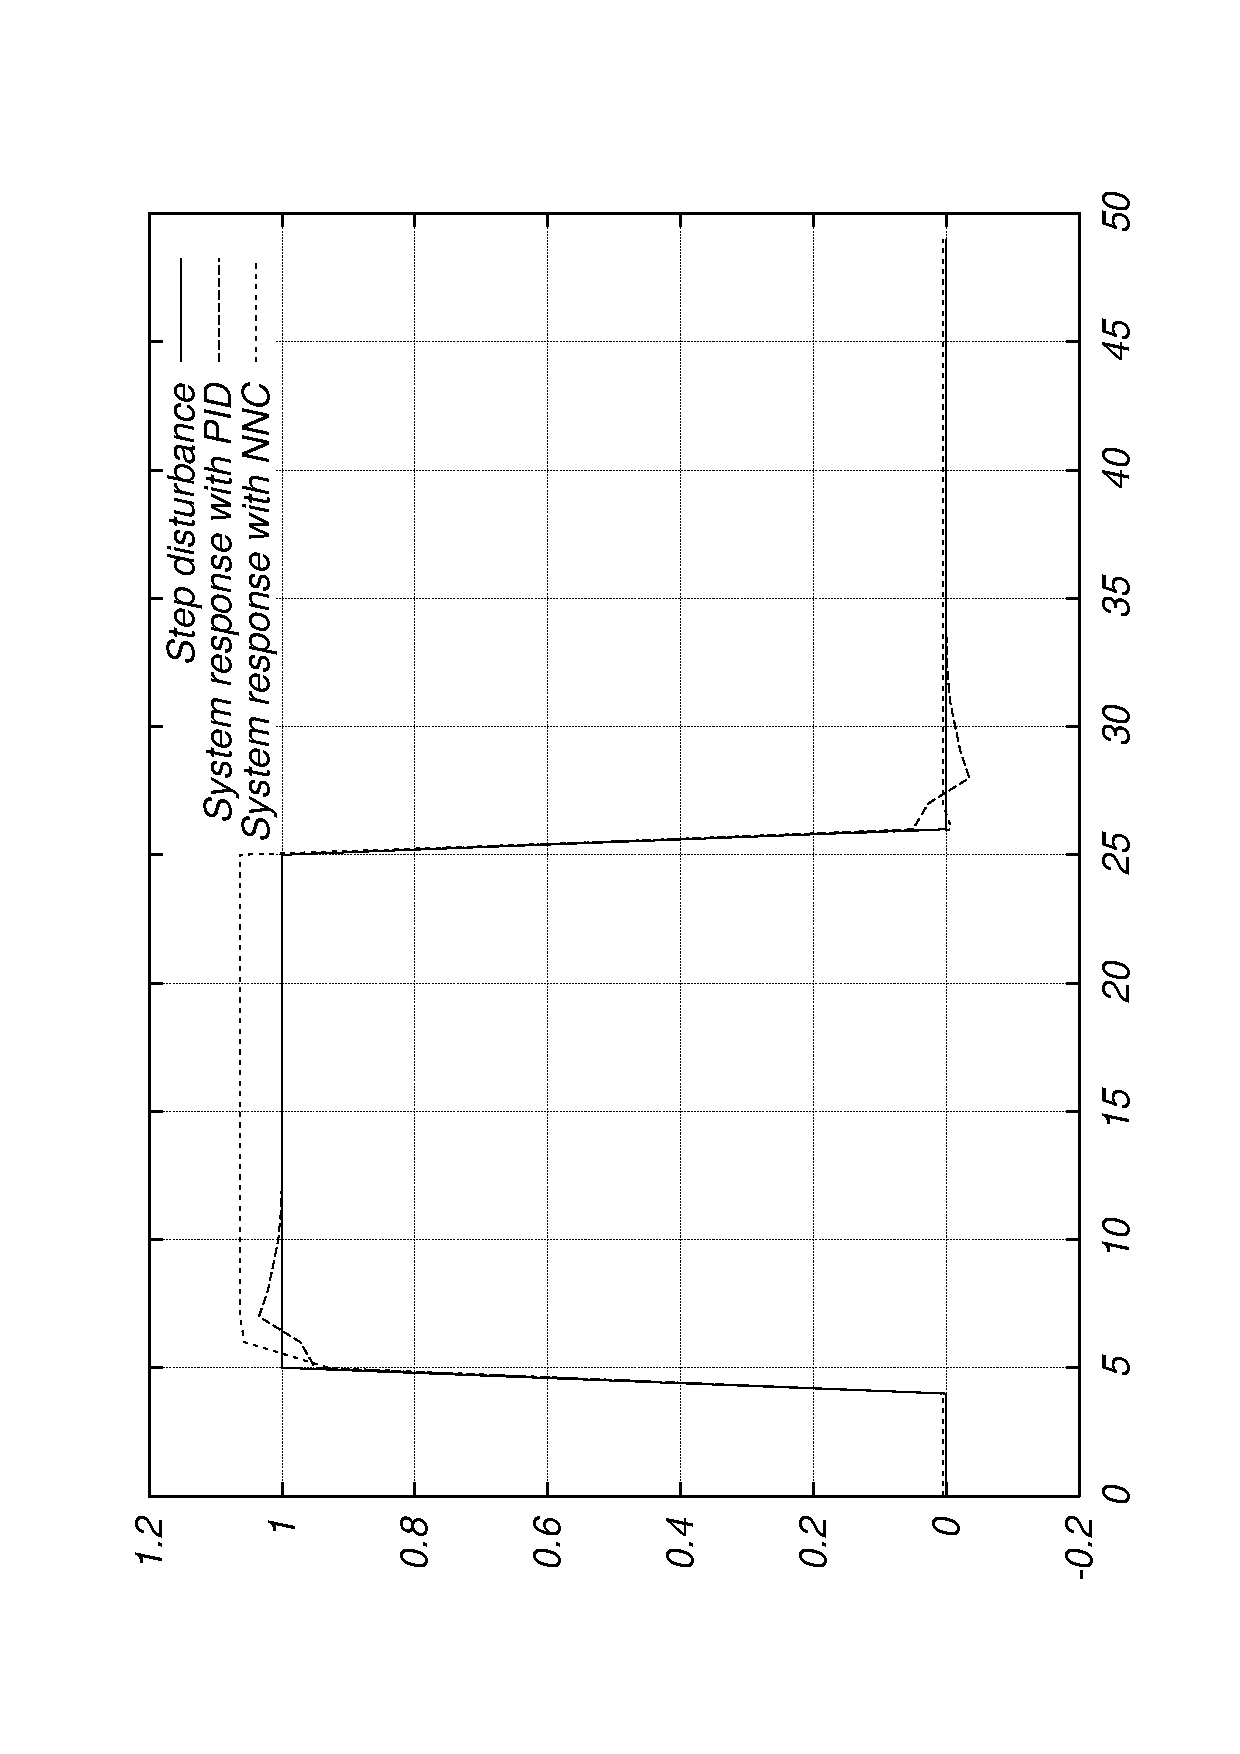
\includegraphics[angle=270,width=0.45\textwidth,%
%             totalheight=0.25\textheight]{pid_npc_step_test} &
%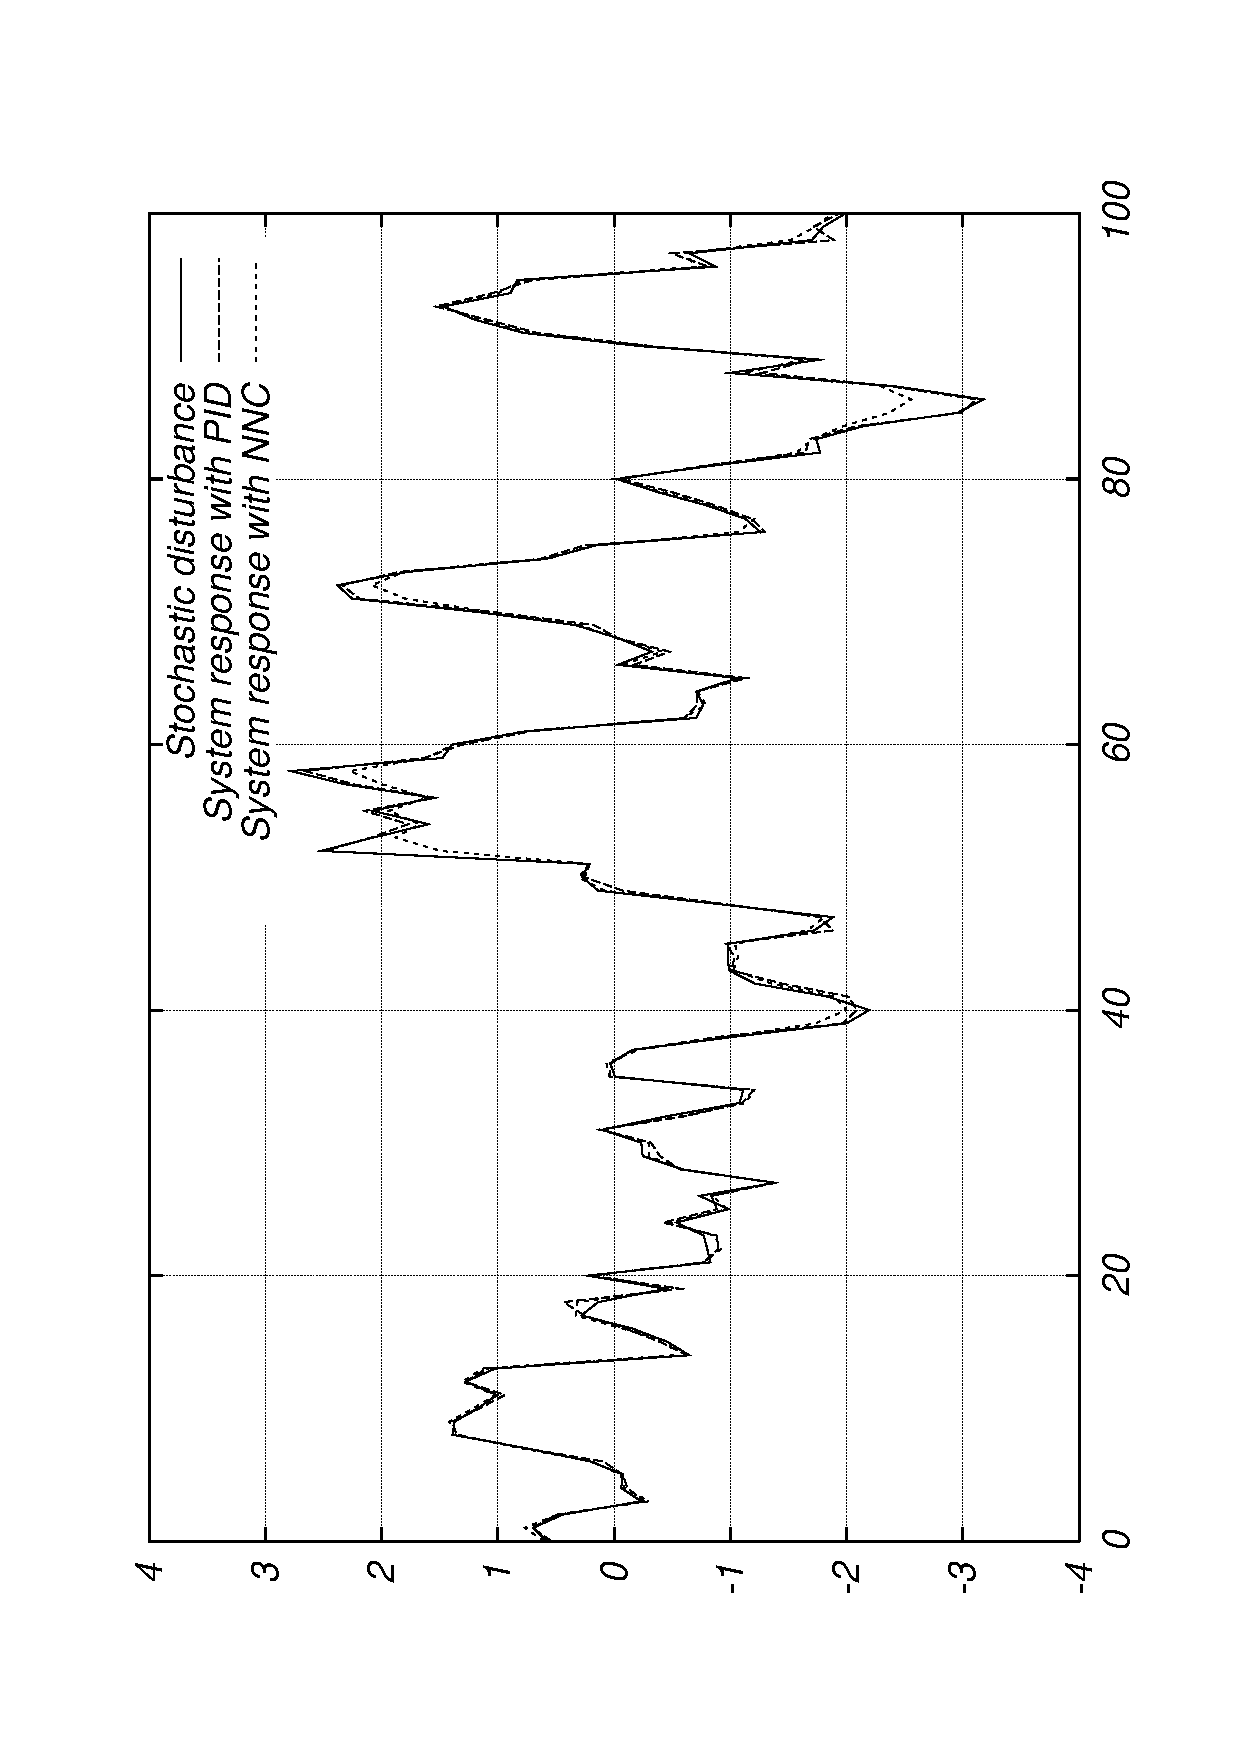
\includegraphics[angle=270,width=0.45\textwidth,%
%             totalheight=0.25\textheight]{pid_npc_stoch_test} \\
%а) & б)\\
%\end{tabular}
%\caption{Отклик системы на прямоугольное (а) и стохастическое (б)
%         возмущающее воздействие при ПИД и НС регулировании ($r_k,e_k$).}
%\label{fig:pid_npc_test}
%\end{figure}

%Рассмотрим значимость последних двух эффектов и способы их
%устранения.

%\paragraph{Статическая ошибка НС--Р}\label{nnc_static_error}
%Эффект статической ошибки был рассмотрен при обучении нейросетевой
%модели объекта управления.  Он связан с различием формы обучающего и
%контрольного сигнала.  В частности, статическая ошибка будет возникать
%на ступенчатой уставке в том случае, если нейросетевой регулятор был
%обучен на стохастическом сигнале уставки.  Эффект статической ошибки
%нейронной сети, как отмечалось на \pgref{amplify-zero}, проявляет себя
%на ступенчатом контрольном сигнале уставки усилением нуля и ошибочным
%коэффициентом передачи.  Отмечается, что для компенсации этого
%нежелательного эффекта можно использовать параллельно с нейросетевым
%линейный регулятор~\cite{steck96}.  Далее рассмотрим способы
%устранения эффекта статической ошибки, не требующие в включения в
%контур управления дополнительных узлов.

%Если условия нормальной эксплуатации регулятора в контуре управления
%характеризуются кусочно-постоянной уставкой, рекомендуется для
%настройки НС--Р взять обучающую выборку, имеющую подобный вид.  В этом
%случае нейросетевая аппроксимация поведения ПИД регулятора будет более
%качественной.  Однако полностью устранить этим способом эффект
%статической ошибки не всегда удается.

%Значительно лучший результат дает подход, основанный на предположении
%о симметрии функций $u_{PID}(t)$ при симметрии функций $r(t)$, $e(t)$
%относительно нуля (или любого другого известного постоянного среднего
%значения).  В этом случае задача аппроксимации для нейронной сети
%упрощается, так как отпадает потребность в пороге --- весовом
%коэффициенте $w_0$ (см. формулу \eqref{eq:neuron_output}), ---
%предназначенном для смещения рабочей области функции активации.
%Функционирование нейрона в этом случае определяется уравнением

%\begin{equation}\label{eq:neuron_output_nobias}
%y=\fa(\sum_{j=1}^nw_j x_j)
%\end{equation}

%После предварительного обучения НС--Р с нулевым порогом на
%стохастическом обучающем множестве контрольная проверка на единичной
%ступени показала уменьшение эффекта статической ошибки по сравнению со
%случаем использования обычных нейронов со смещением $w_0$
%(\figref{fig:npc_static_error}).  В частности, ошибка в имитации
%коэффициента передачи уменьшилась с 6\% до 4.5\%, а эффект усиления
%нуля уменьшился до исчезающе малых величин.

%\begin{figure}[h]
%\centering
%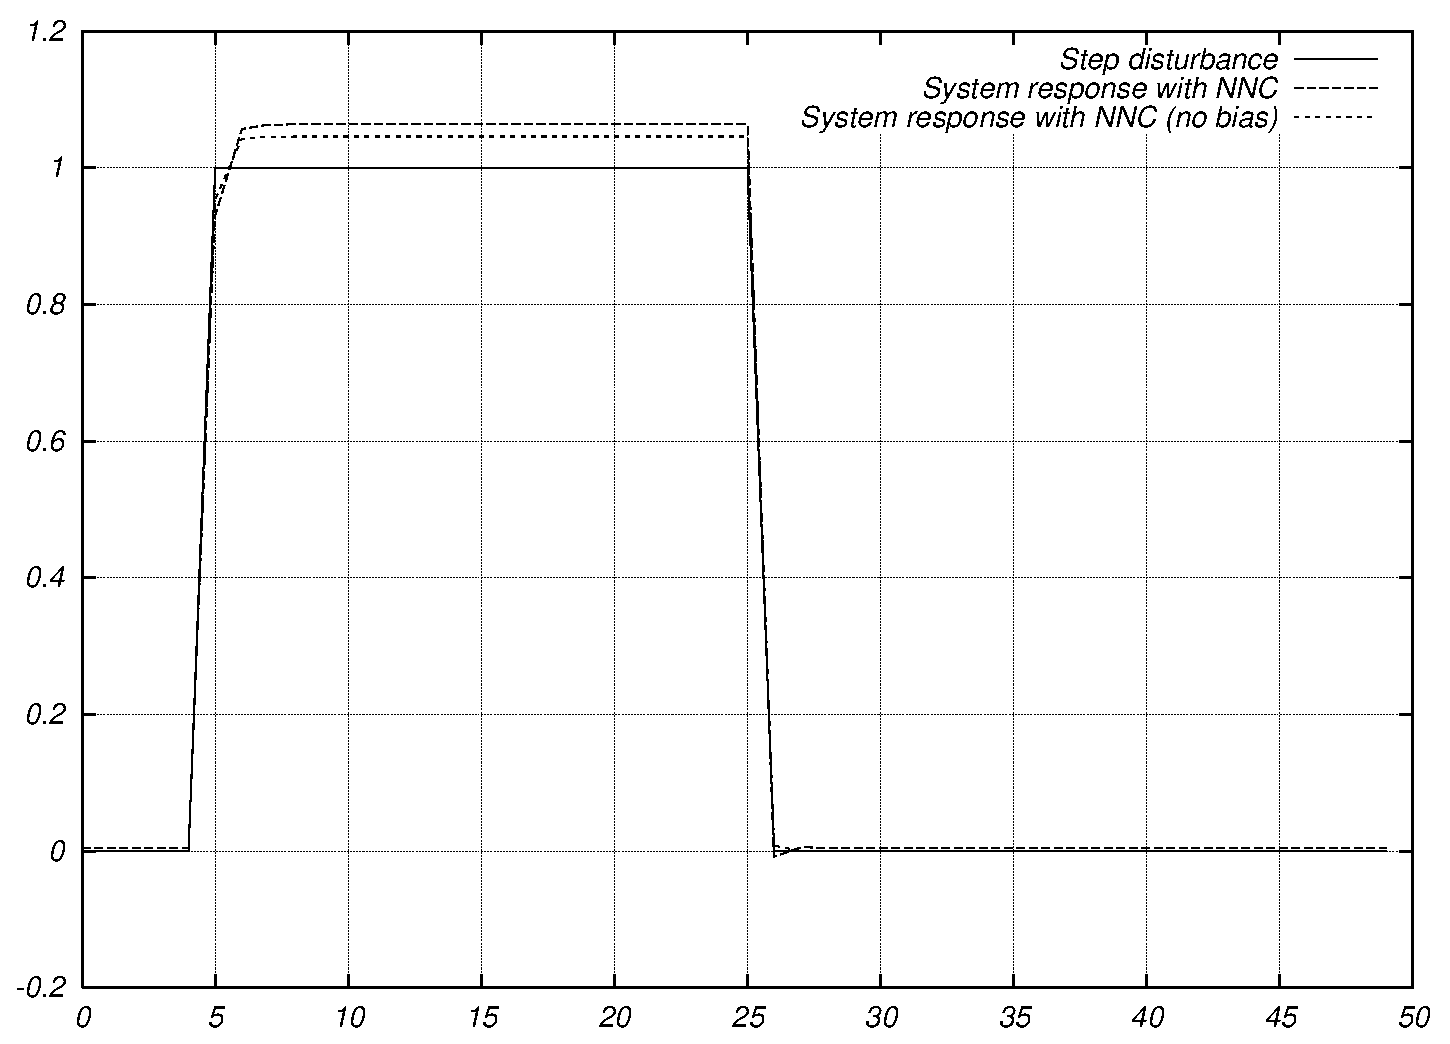
\includegraphics[angle=270,width=0.8\textwidth,%
%             totalheight=0.35\textheight]{npc_nob_step_test}
%\caption{Эффекты статической ошибки НС--Р в случаях наличия смещения $w_0$ у
%         нейронов сети и в случае его отсутствия.}
%\label{fig:npc_static_error}
%\end{figure}

%Следует отметить, что эффект статической ошибки проявляет себя в
%основном на участках постоянной уставки при полном отсутствии помех.
%В случае наличия постоянных изменений на входах НС--Р, которые могут
%быть вызваны изменениями уставки или шумом в канале наблюдения, эффект
%статической ошибки себя не проявляет.  Это означает отсутствие
%различий между исходным ПИД регулятором и предварительно обученным
%нейросетевым.  Подобным может считаться случай синтеза Винеровского
%оптимального регулятора вследствие наличия случайных помех и
%стохастической природы уставки.

%\subsection{Внутренняя структура нейросети}

Исследуем влияние количества скрытых слоёв и нейронов в них на
процесс обучения и качество имитации исходного регулятора.  Для этого
возьмем несколько нейронных сетей с входами $r_k,e_k$ и количеством
скрытых слоёв от 0 до 3 и обучим их на одних и тех же данных.  В
качестве обучающего множества будем использовать выборку длиной 800
отсчетов, а в качестве контрольной --- длиной 200 отсчетов.  Обе
выборки получены при стохастической уставке и случайной помехе.

Продолжительность пакетного обучения НС--Р измерялась в эпохах за
которые достиглась ошибка заданного уровня (в проведенных
экспериментах был взят уровень 0.006).  Если за 3000 эпох ошибка всё
ещё была больше заданного уровня, то обучение останавливалось на
достигнутом результате.  После обучения НС--Р включался в контур
управления и в условиях отсутствия помехи на вход системы поступала
ступенчатая уставка.  Качество управления оценивалось по
среднеквадратической ошибке управления на ступенчатой уставке.
Результаты эксперимента приведены в \tablref{tabl:nnc_internal_arch}.

\begin{table}
\caption{Влияние внутренней структуры НС--Р на обучение и качество имитации.}\label{tabl:nnc_internal_arch}
\begin{tabular}{|l|c|c|c|c|}
\hline
$\mathrm{N}^o$ & Архитектура НС--Р & Ошибка обучения & Ошибка управления & Время вычислений, с\\
\hline
1 & $\NN^p_{r+e,1}$          & 0.0066& 0.0058 & 57.0\\
2 & $\NN^p_{r+e,5,1}$        & 0.0065& 0.0061 & 76.2\\
3 & $\NN^p_{r+e,20,1}$       & 0.0065& 0.0060 & 132.1\\
4 & $\NN^p_{r+e,7,5,1}$      & 0.0067& 0.0061 & 120.2\\
5 & $\NN^p_{r+e,20,10,1}$    & 0.0067& 0.0063 & 306.6\\
6 & $\NN^p_{r+e,7,9,5,1}$    & 0.0070& 0.0062 & 194.4\\
7 & $\NN^p_{r+e,15,20,10,1}$ & 0.0067& 0.0064 & 571.1\\
\hline
\end{tabular}
\end{table}

На основании проведенных экспериментов можно сделать вывод, что
внутренняя структура многослойного персептрона НС--Р с входами
$r_k,e_k$ не оказывает значительного влияния на качество имитации ПИД
регулятора, управляющего линейным объектом.  В то же время, количество
нейронов в нейронной сети напрямую определяет вычислительную сложность
процесса обучения.  Поэтому усложнение внутренней архитектуры НС--Р
увеличивает время вычислений, а также может привести к потере сетью
обобщающей способности.  Очевидно, в такой ситуации предпочтительнее
использовать более простые архитектуры.  Однако, следует иметь в виду,
что возможность нейросетевой аппроксимации произвольной функции
доказано только для сетей с не менее чем двумя слоями нелинейных
нейронов.  Это особенно важно если априорно известно о нелинейности
объекта управления.

\section{Обучающие данные}

Обучение искусственной нейронной сети с учителем требует наличия
набора данных, определяющих эталонные пары вход-выход.  Для
нейросетевого регулятора с комбинированным управлением по возмущению и
отклонению входом является пара $r_k,e_k$, а выходом --- управляющее
воздействие исходного регулятора $u_k$.  Эти данные легко получить при
наблюдении за функционированием системы управления.  Однако возникает
вопрос об оптимальном объёме данных, а также о наилучшем пробном
сигнале для обучения НС--Р.

%\subsection{Вид пробного сигнала}

При настройке линейных регуляторов (в частности, ПИД) в контуре, как
правило, используются детерминированные сигналы уставки ступенчатой
или гармонической формы.  В то же время, в процессе работы уставка
обычно изменяется случайным образом.  Исследуем в эксперименте, какой
из перечисленных трех видов уставки обеспечивает обучение НС--Р для
наилучшей имитации исходного регулятора.  Для этого сгенерируем
временные ряды одинаковой длительности $L=2000$: меандр,
моногармонический сигнал и цветной шум (формирующая функция
$R^*(z)=\frac{0.625z}{z-0.779}$).  Фрагмент полученных рядов уставки
приведен на~\figref{fig:probe_signals}.  В числе внешних воздействий
на систему кроме уставки имеет место случайная помеха в канале
наблюдения.  В эксперименте она является нормально распределенным
белым шумом с нулевым средним и дисперсией 0.01.

\begin{figure}
\centering
\includegraphics[width=0.8\textwidth,%
  totalheight=0.35\textheight]{probe_signals_rus}
\caption{Временные ряды уставки разных видов.}\label{fig:probe_signals}
\end{figure}

По плану эксперимента уставка выбранного вида подавалась на вход
системы управления с исходным ПИД регулятором, после чего временные
ряды ошибки управления $e(t)$ и управляющего воздействия $u(t)$
сохранялись.  С их помощью осуществлялась настройка НС--Р с
архитектурой $\NN^p_{r+e,5,1}$.  Обученный НС--Р помещался на место
исходного ПИД регулятора в контур управления и на вход системы
подавалась ступенчатая уставка.  Для лучшей иллюстративности помеха в
систему не подавалась.  Наилучшее качество имитации ПИД регулятора
должно обеспечивать наилучшее качество управления: величину
перерегулирования, время затухания переходного процесса.

Результаты управления настроенных НС--Р в контуре показан
на~\figref{fig:nnc_system_response}.  Видно, что наихудшим оказался
НС--Р, настроенный на ступенчатой уставке, так как он привел к
высокочастотным осцилляциям в системе без каких-либо признаков
стабилизации состояния объекта.  НС--Р, обученный на гармонической
уставке, обеспечил управление объектом, однако величина
перерегулирования, время переходного процесса и остаточная ошибка при
постоянном уровне уставки достаточно велики.  Наилучший результат
показал НС--Р, настроенный на стохастической уставке.  При чуть
меньшем перерегулировании он обеспечил гораздо более короткий
переходный процесс и существенно меньшую остаточную ошибку.  Результат
работы этого нейросетевого регулятора в сравнении с исходным ПИД
показан на \figref{fig:nnc_pid_system_responses}.

\begin{figure}
\centering
\includegraphics[width=0.8\textwidth,%
  totalheight=0.35\textheight]{nnc_system_response_rus}
\caption{Результат работы НС--Р, настроенного на обучающих данных с уставкой
         разных видов.}\label{fig:nnc_system_response}
\end{figure}

\begin{figure}
\centering
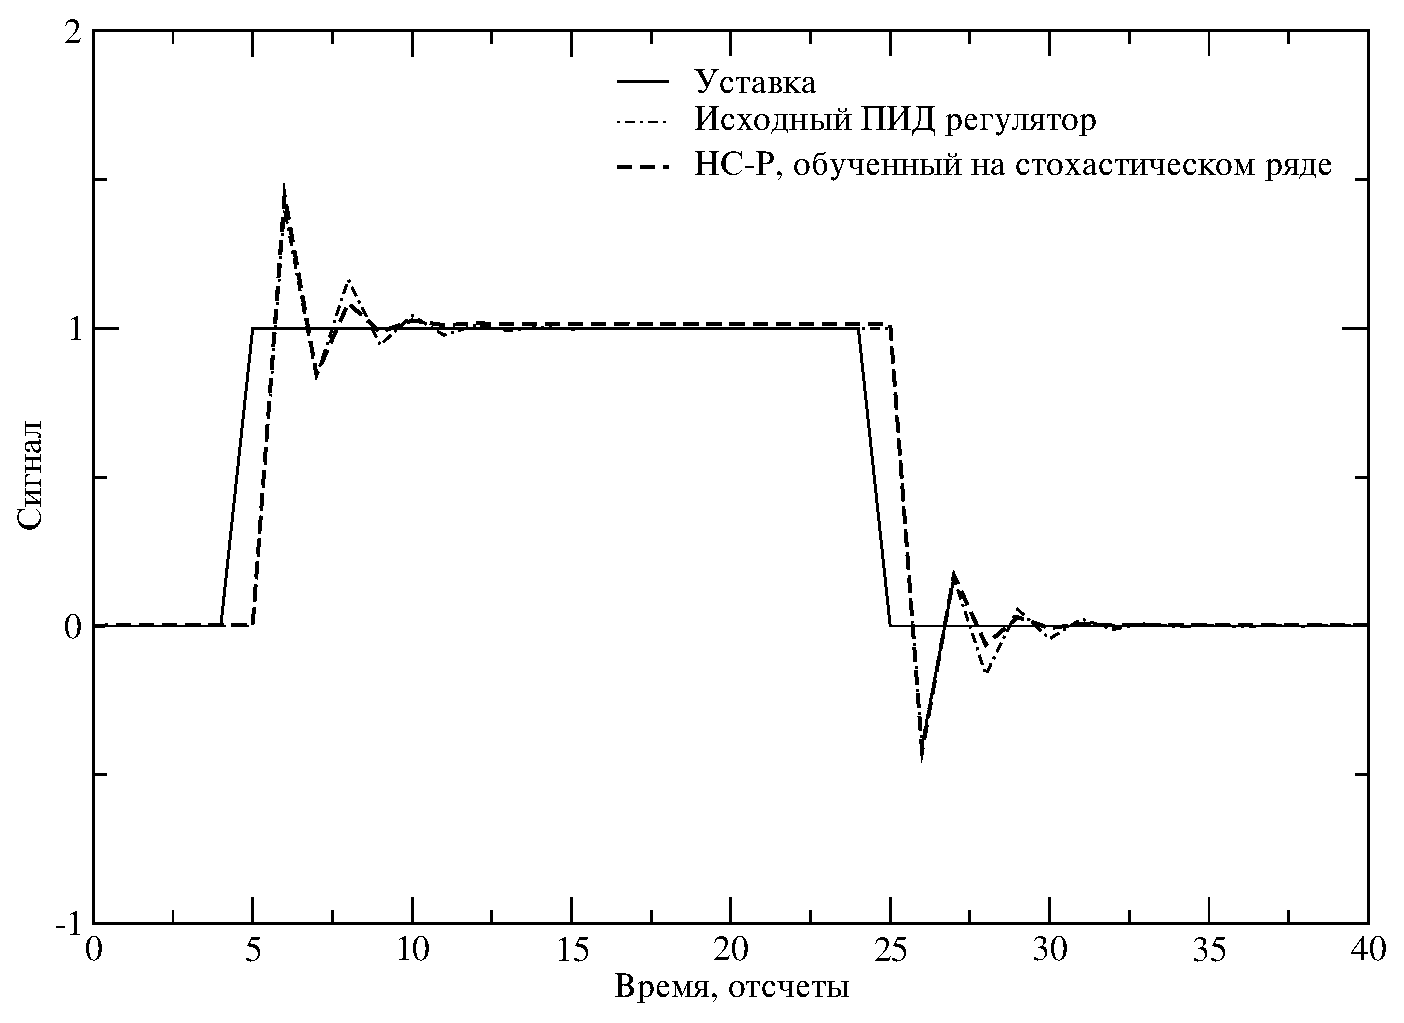
\includegraphics[width=0.8\textwidth,%
  totalheight=0.35\textheight]{nnc_pid_system_responses_rus}
\caption{Сравнение работы исходного ПИД регулятора с лучшим НС--Р.}%
\label{fig:nnc_pid_system_responses}
\end{figure}

Если для обучающей выборки целесообразно использовать стохастическую
уставку, то для контрольной выборки лучше всего взять уставку,
наиболее типичную для данной системы автоматического регулирования.

%\subsection{Объём обучающих данных}

Причины значительного преимущества стохастических пробных сигналов
перед детерминированными кроются в более равномерном покрытии области
определения функции нейронной сети обучающими точками.  Для НС--Р
рассматриваемой архитектуры входное множество двумерное и оно
образуется парами $r_k,e_k$.  Плотность покрытия обучающими точками
для трех видов уставок, участвовавших в эксперименте, приводится
на~\figref{fig:probe_signals_re2d}.  Видно, что обучающие точки,
полученные при периодической ступенчатой уставке, сгруппированы на
очень малой площади.  Гармоническая уставка дает более равномерное
распределение, но её периодичность проявляется областями чрезмерной
концентрации обучающих точек, регулярно расположенных на плоскости.
Стохастическая уставка обеспечивает покрытие плоскости $r\times e$
обучающими точками по закону распределения, близкому к двумерному
нормальному.  В эксперименте получена следующая приблизительная оценка
покрытия обучающими точками рабочей части плоскости $r\times e$
(диапазон уставок $[-3,3]$, диапазон ошибок $[-2,2]$): уставка-меандр
дает 14\% покрытия, моногармоническая уставка --- 43\%, стохастическая
--- 72\%.  Очевидно, что в последнем случае обучение нейронной сети
для рабочей части плоскости будет наиболее полноценным.

\begin{figure}
\centering
\begin{tabular}{c}
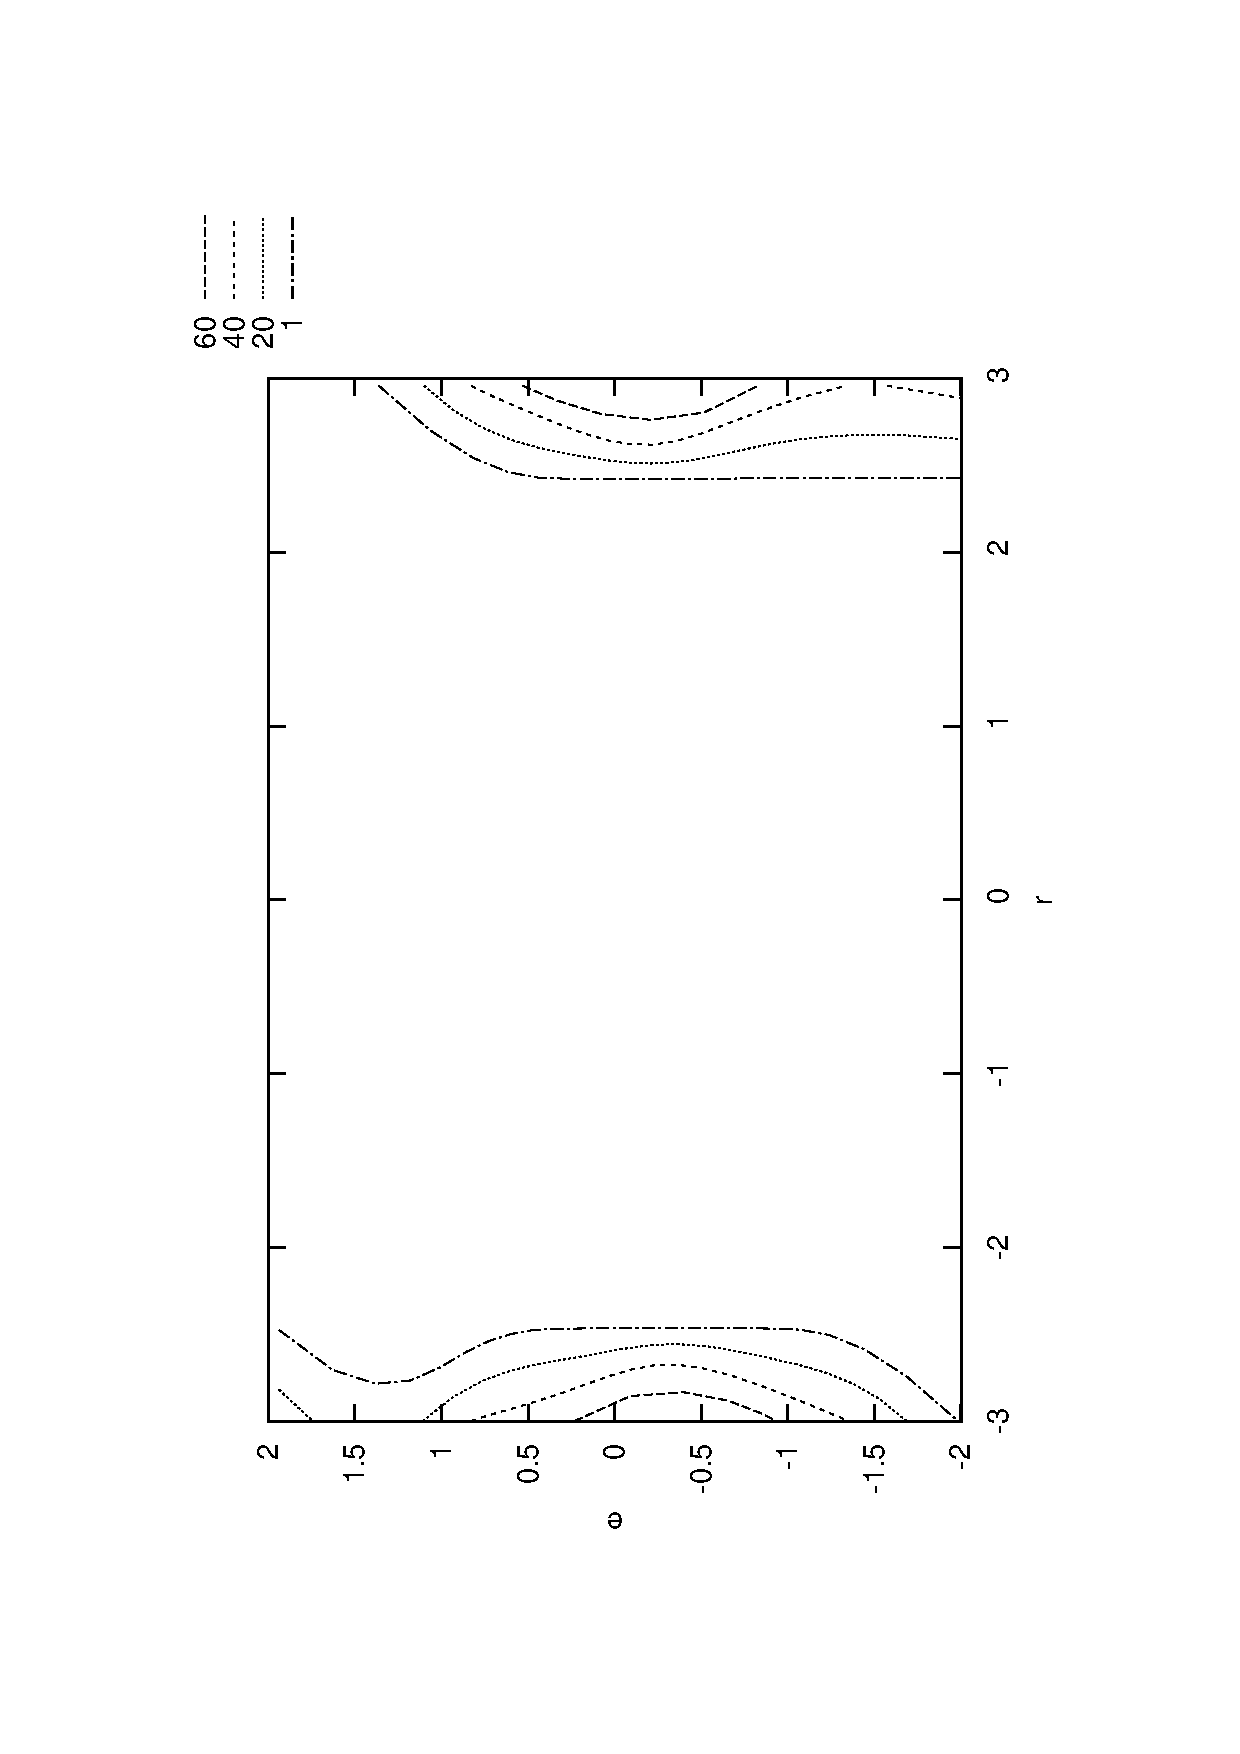
\includegraphics[angle=270,width=0.6\textwidth,%
  totalheight=0.25\textheight]{step_re2d}\\
а)\\
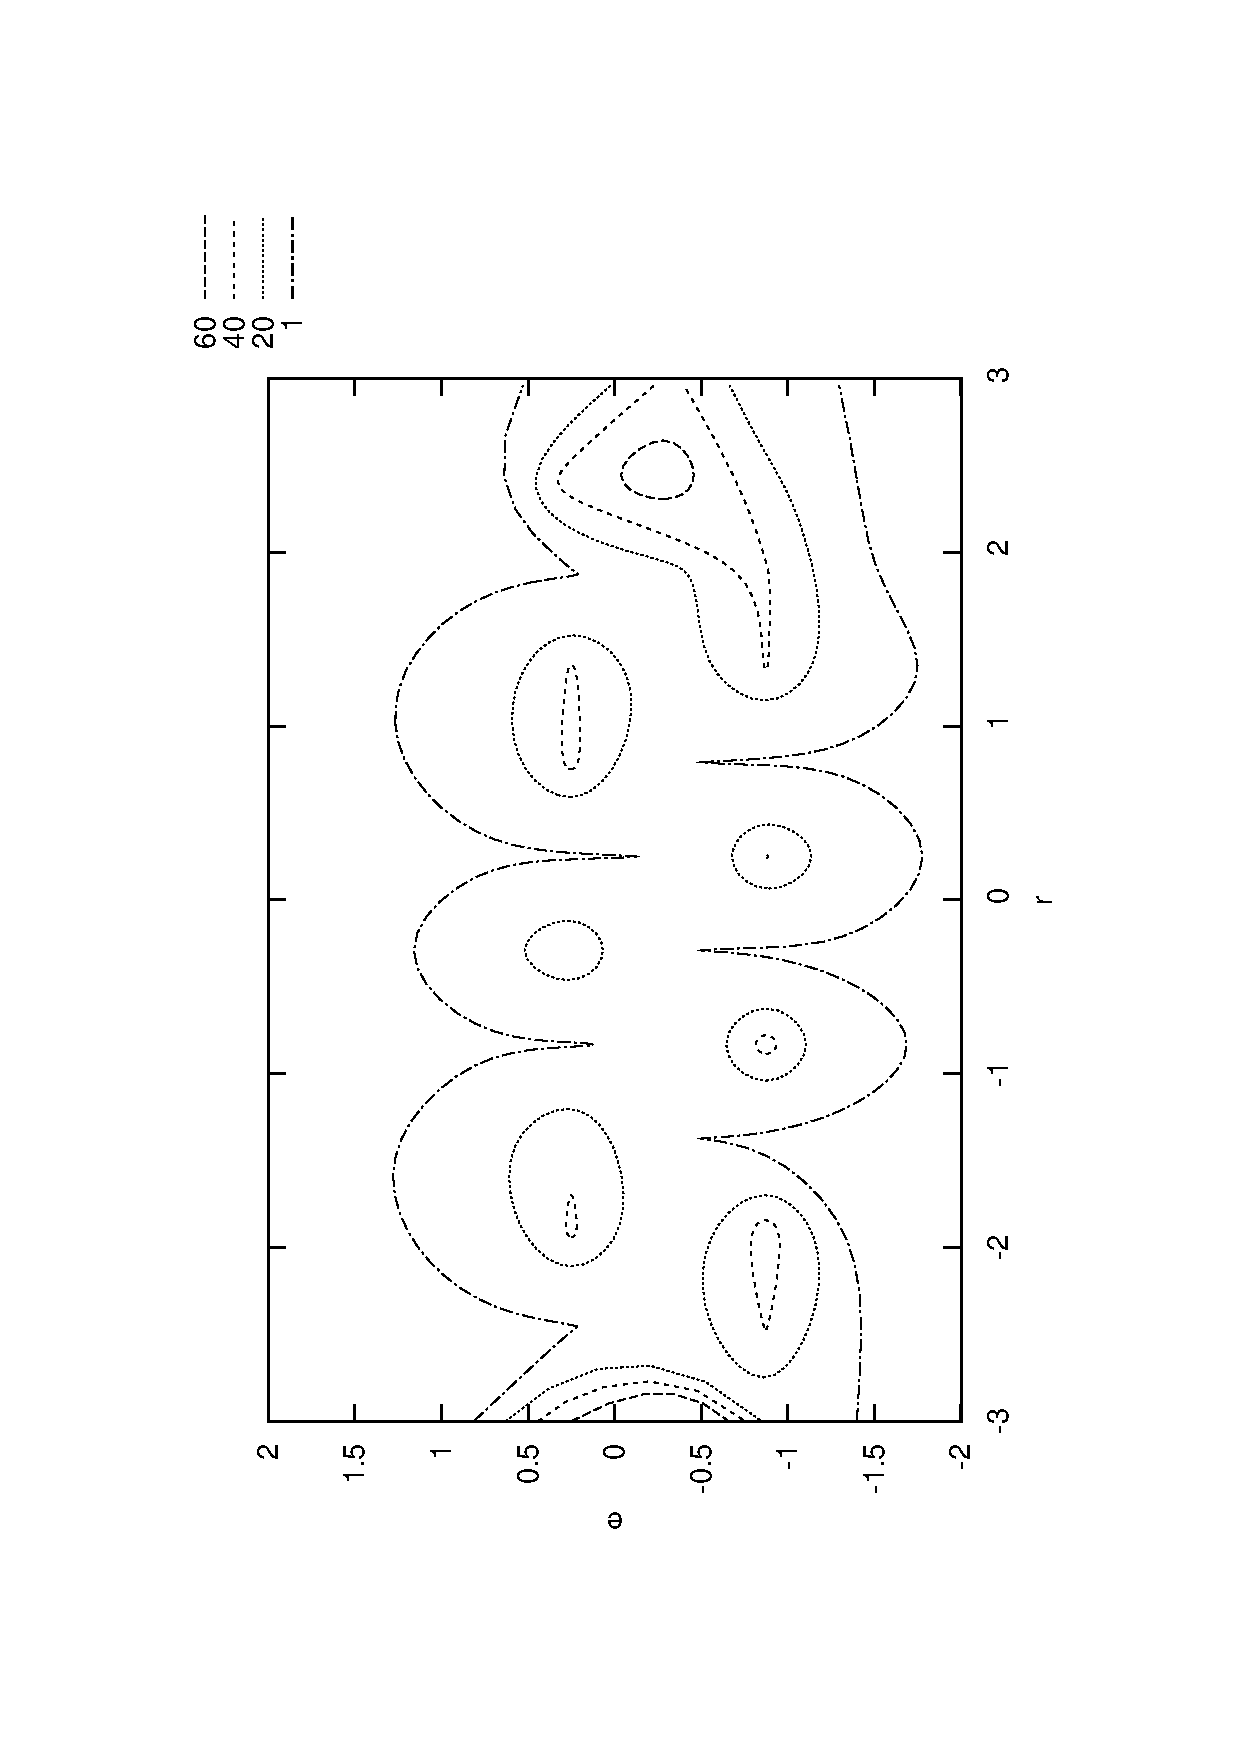
\includegraphics[angle=270,width=0.6\textwidth,%
  totalheight=0.25\textheight]{harm_re2d}\\
б)\\
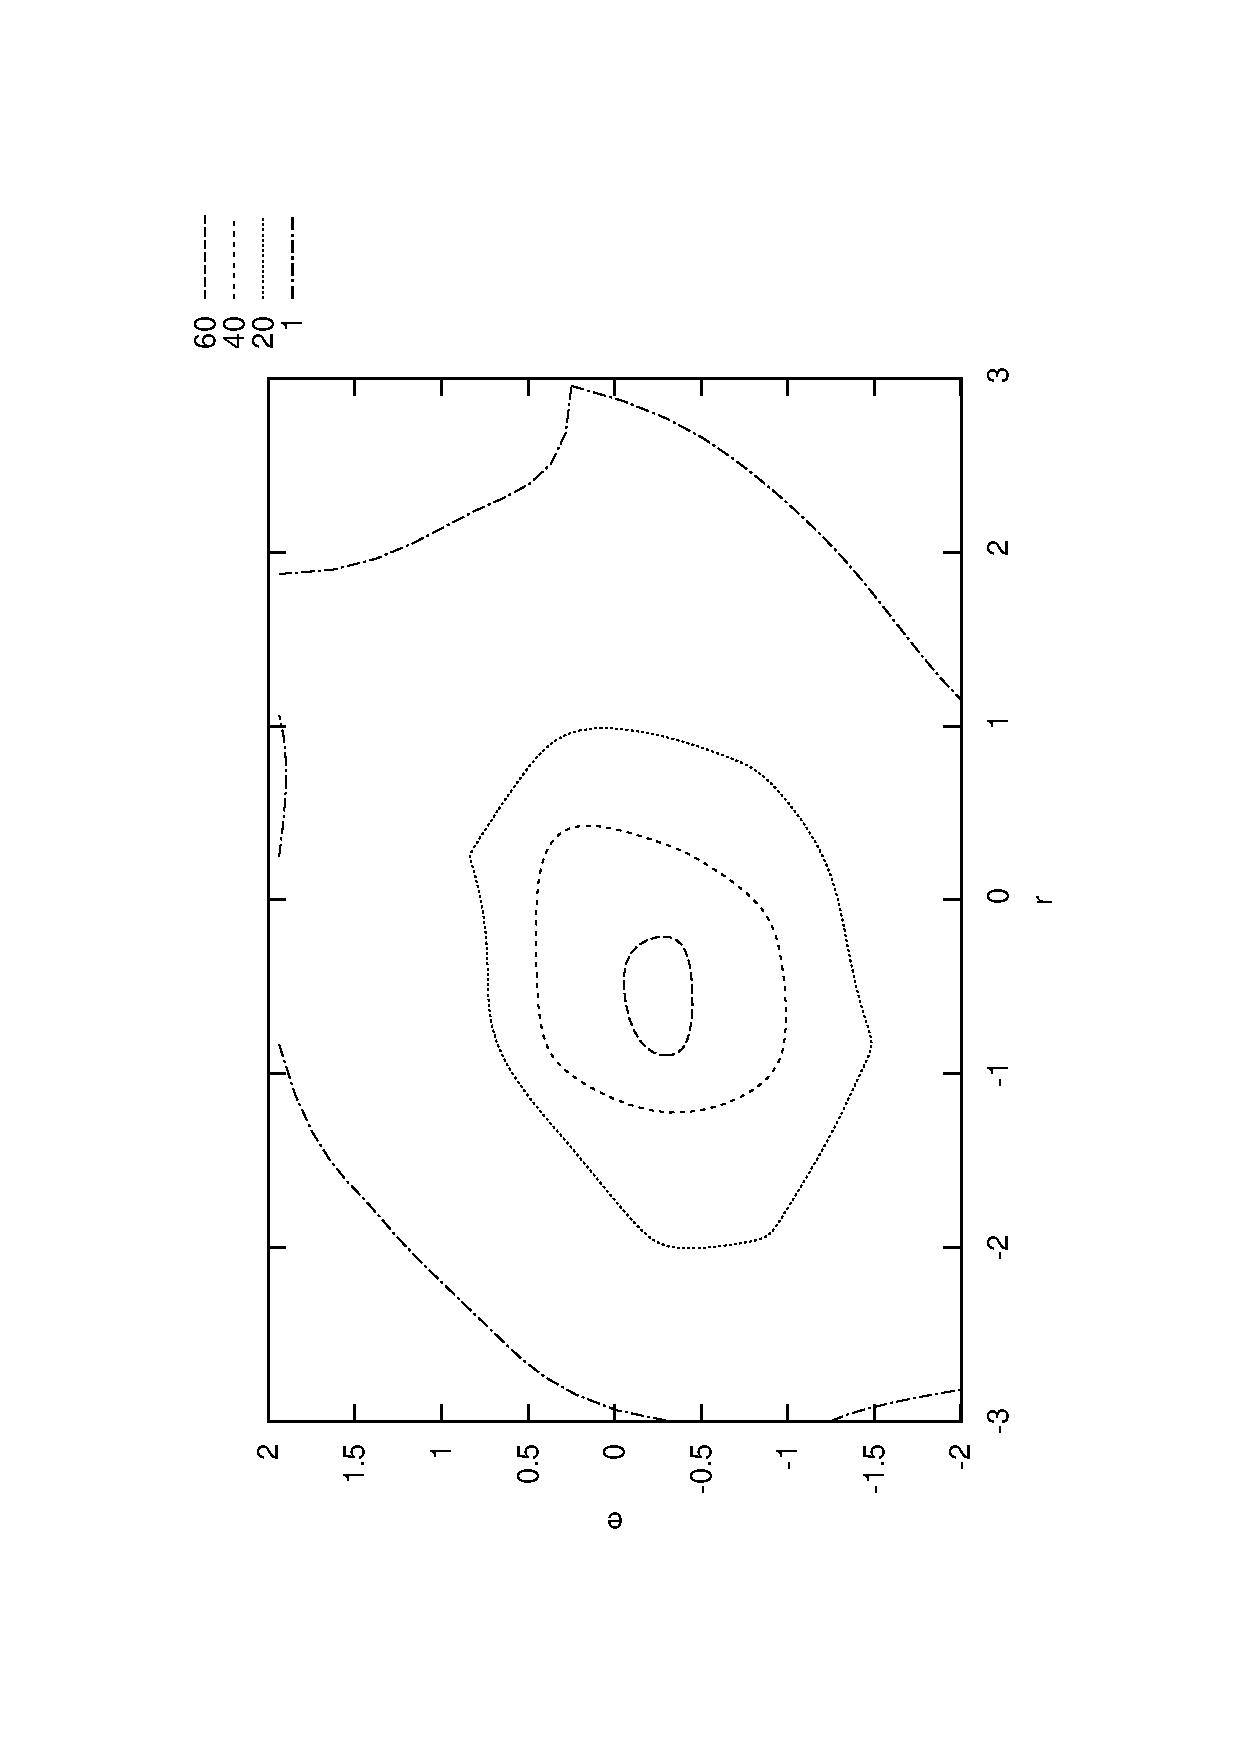
\includegraphics[angle=270,width=0.6\textwidth,%
  totalheight=0.25\textheight]{stoch_re2d}\\
в)\\
\end{tabular}
\caption{Распределение обучающих точек на плоскости $r\times e$
         при ступенчатой периодической (а), моногармонической (б) и
         стохастической уставке (в).}%
\label{fig:probe_signals_re2d}
\end{figure}

Для обозначения границ, в пределах которых нейронная сеть
функционирует с эффективностью, полученной при обучении удобно ввести
термин --- {\em область гарантированного качества}.  Данное понятие
легко конкретизируется на случай обучения нейросетевого регулятора:
если для системы управления известны диапазоны допустимых (или
возможных) уставки и ошибки управления, область гарантированного
качества НС--Р должна охватывать как можно большую часть этих
диапазонов.  Для обеспечения этого требования множество обучающих
данных, полученных на исходной системе управления, должно покрывать
как можно большую часть рабочих диапазонов уставки и ошибки
управления.

Если рабочие диапазоны не заданы, можно оценить параметры
распределения уставки и ошибки накапливать данные в обучающем
множестве до тех пор, пока наиболее вероятный диапазон значений не
будет заполнен с желаемой плотностью.  Плотность обучающих пар должна
быть тем выше, чем больше нейронов (весовых коэффициентов) имеется в
нейронной сети регулятора.

\section{Обучение нейронной сети регулятора и контроль качества имитации}

%\paragraph{Описание схемы обучения с учителем}
После выбора архитектуры нейронной сети регулятора встает задача его
обучения, то есть, настройки весовых коэффициентов нейронов с целью
как можно более точного копирования поведения исходного регулятора.
Взяв за основу среднеквадратический критерий,
имеем~\eqref{eq:nnp_synthesis_task}.  Опираясь на рекомендации
относительно выбора входов нейронной сети, можно уточнить, что
$\mathbf{i}_k=[r_k,e_k\ldots e_{k-d}]$, где $d$ --- величина памяти
прошлых значений ошибки.  Введя для удобства обозначения для выхода
эталонного регулятора $u_k=f(e_k,\mathbf{s})$ и нейросетевого
$\hat{u}_k=\NN^p(r_k,e_k\ldots e_{k-d})$, имеем:
\begin{equation}\label{eq:nnc-learning-criterium}
  \sum\limits_k\big(u_k-\hat{u}_k\big)^2\rightarrow\min
\end{equation}

Для многослойного персептрона со слоями $1<L<L_{out}$, взятого за
основу НС--Р, обучение с учителем предлагается проводить градиентным
методом.  Например, для обратного распространения ошибки, методика
обучения представлена следующими уравнениями:
\begin{equation}
  \label{eq:sigm_neuron_output_parts}
  \begin{array}{rcll}
    z^L_i & = & \sum\limits_j w^L_{ij}q^{L-1}_j & 1<L\le L_{out}\\
    q^L_i & = & \fa(z^L_i), & \\
  \end{array}
\end{equation}причем $\hat{u}_k=q^{L_{out}}_i$.

Входы $r_k,e_k\ldots e_{k-d}$ нейронной сети регулятора отображаются
на $q^1_j$ по следующему правилу:
\begin{equation}
  q^1_j =\left\{
  \begin{array}{ll}
    r_k & j=1 \\
    e_{k-j+2} & 2\le j\le d+2 \\
  \end{array}\right.
\end{equation}

Обобщенная ошибка $\delta^L_i$ в $i$-ом нейроне слоя $L$ от выходов
НС--Р к входам вычисляется в соответствии с уравнениями:
\begin{equation}\label{eq:nnc-generalized-error}
  \delta^L_i=\left\{
  \begin{array}{ll}
    \fa'(z^L_i)\sum\limits_h\delta^{L+1}_h w^{L+1}_{hi} & 1\le L<L_{out} \\
    \fa'(z^L_i)(\hat{u}_k-u_k) & L=L_{out} \\
  \end{array}\right.
\end{equation}

%{\LARGE УБРАТЬ!!!}
%\begin{equation}
%  \delta^L_i=\left\{
%  \begin{array}{ll}
%    \fa'(z^L_i)\sum\limits_h\delta^{d+1}_h w^{d+1}_{hi} & 1\le d<d_{out} \\
%    \fa'(z^L_i)(y_k-\hat{y}_k) & d=d_{out} \\
%  \end{array}\right.
%\end{equation}
%\begin{equation}
%  \hat{\mathbf{y}}_k=\NN(\mathbf{x}_k)
%\end{equation}
%\begin{equation}
%  q^0_j\equiv x_j
%\end{equation}
%\begin{equation}
%  w^L_{ij}(k+1)=w^L_{ij}(k)-\eta\delta^L_i q^{L-1}_j
%\end{equation}

Коррекция весовых коэффициентов $i$-го нейрона на основе рассчитанной
обобщенной ошибки, $j$-го входа нейрона и коэффициента скорости
обучения $\eta$ осуществляется по дельта-правилу:
\begin{equation}\label{eq:nnc-weights-update}
  w^L_{ij}(k+1)=w^L_{ij}(k)-\eta\delta^L_i q^{L-1}_j
\end{equation}

%\paragraph{Упомянуть об особенностях градиентных методов (ссылки)}
Описанный подход к обучению является градиентным методом первого
порядка, что обуславливает, с одной стороны, его простоту и
нетребовательность при реализации, с другой стороны, малую скорость
сходимости.  В литературе описаны многочисленные методы обучения
нейронных сетей, в том числе, методы, использующие приближения второго
порядка, дающие большую скорость сходимости.  Среди них методы
быстрого распространения (QuickProp), сопряженных градиентов,
Левенберга-Маркварта и др.~\cite{osov04,haykin2008,gibb96}.  При всех
достоинствах перечисленных методов все они имеют общий родовой
недостаток с методом обратного распространения ошибки: возможность
нахождения локального, а не глобального минимума.  Это является
следствием локальности градиентных методов оптимизации.

В качестве альтернативы градиентным методам иногда используются методы
нелокальной оптимизации, в частности, больцмановский метод и метод
искусственной теплоемкости~\cite{wasser92,golovko01}, однако они дают
худшую скорость обучения, чем градиентные.

В ряде экспериментах было установлено, что для задачи имитации ПИД
регулятора нейросетевым скорости сходимости метода обратного
распространения вполне достаточно даже при использовании не самых
быстродействующих персональных компьютеров.  Находимые в процессе
обучения решения обеспечивали удовлетворительную ошибку, что может
являться свидетельством гладкости гиперповерхности ошибки в
пространстве весовых коэффициентов на задачах рассматриваемого класса.

%\subparagraph{Пакетное обучение}

Процедура обучения, описанная уравнениями
\eqref{eq:nnc-learning-criterium}--\eqref{eq:nnc-weights-update},
проводится на обучающей выборке
$\mathbf{R}^T,\mathbf{E}^T,\mathbf{U}^T$, то есть, $\forall
r_k\in\mathbf{R}^T, e_k\in\mathbf{E}^T, u_k\in\mathbf{U}^T$.  При этом
используется так называемое пакетное обучение ({\em batch learning}),
при котором обобщенная ошибка~\eqref{eq:nnc-generalized-error}
вычисляется для каждого элемента $r_k,e_k,u_k$ обучающей выборки, а
коррекция весовых коэффициентов производится только после предъявления
всех элементов из обучающей выборки~\eqref{eq:nnc-weights-update}.
Шаг процедуры обучения между коррекциями весовых коэффициентов
называется эпохой ({\em epoch}).  Пакетное обучение имеет следующие
преимущества перед более частым обновлением весовых коэффициентов:
\begin{itemize}
\item При влиянии помех на исходную систему управления обучающая
  выборка также будет искажена помехами.  Если считать помеху
  случайной величиной с нулевым математическим ожиданием, то
  использование пакетного обучения позволяет минимизировать влияние
  помехи на рассчитанные поправки весовых коэффициентов.
\item Направление изменения весовых коэффициентов определяется всей
  обучающей выборкой, что предохраняет процесс обучения от
  ``рыскания'', вызыванного отдельными незакономерными её элементами.
\end{itemize}

%\paragraph{Используемые эвристики}

%\subparagraph{Различие $\eta$ и $\eta_out$}
%При обучении коэффициент скорости обучения $\eta$ различался для
%скрытых слоёв $\eta_{hidden}$ и для выходного слоя (нейрона)
%$\eta_{output}$, причем обычно выбиралось соотношение
%$2<\eta_{hidden}/\eta_{output}\le 10$.  Таким образом, изменение
%весовых коэффициентов выходного нейрона намеренно тормозилось по
%сравнению с остальными нейронами.  Это делалось специально, так как 

В процессе обучения коэффициент скорости изменялся по следующему правилу:
\begin{itemize}
\item Если на протяжении 10 эпох среднеквадратическая ошибка на
  обучающей выборке уменьшалась, то коэффициент скорости обучения
  увеличивался на 10\%.
\item Если по окончании эпохи среднеквадратическая ошибка на обучающей
  выборке увеличилась, то весовые коэффициенты нейросети возвращались
  к предыдущему состоянию, а эпоха повторялась с коэффициентом
  скорости, меньшим в два раза.
\end{itemize}
Данная эвристика в рамках стандартного алгоритма обратного
распростанения ошибки в автоматическом режиме позволяет управлять
скоростью обучения, что практически позволяет не заботиться о выборе
коэффициента $\eta$.

Кроме обучающей выборки $\mathbf{R}^T,\mathbf{E}^T,\mathbf{U}^T$ в
процедуре обучения принимает участие проверочная выборка
$\mathbf{R}^V,\mathbf{E}^V,\mathbf{U}^V$, которая не принимает участие
в формировании поправок весовых коэффициентов, но по которой в конце
каждой эпохи также рассчитывается среднеквадратическая ошибка.
Независимость проверочной выборки от обучающей позволяет оценивать
обобщающую способность нейронной сети чтобы вовремя диагностировать
эффект переобучения, когда нейронная сеть начинает подстраиваться под
частные особенности обучающей выборки.

Останов процедуры обучения осуществляется по выполнению хотя бы одного
из условий:
\begin{itemize}
\item Достигнут заданный уровень среднеквадратической ошибки на
  тестовой выборке.
\item Зарегистрирован рост среднеквадратической ошибки на тестовой
  выборке на протяжении нескольких эпох.  Это является свидетельством
  начала потери нейросетью свойства обобщения.
\item Достигнуто максимальное количество эпох, заданное перед началом
  обучения.
\end{itemize}

Следует особо отметить, что никакое среднеквадратическое значение
ошибки на обучающей или проверочной выборке, достигнутое в процессе
обучения, не гарантирует хорошее качество имитации в контуре
управления (см., например, далее
\figref{fig:cstr_e5r1_vs_e1r1_training} и
\figref{fig:cstr_pid_vs_nnc_inloop_rus}).  В случае, если качество
имитации в контуре управления оказывает недостаточным, то следует
повторить процедуру синтеза нейросетевого регулятора сначала, проведя
анализ неудачи.  В частности, если обучение НС--Р было остановлено
вследствие потери сетью обобщающей способности, то, возможно, следует
увеличить число входов НС--Р и выбрать более сложную внутреннюю
структуру (больше слоев и нейронов в слоях), а также увеличить объем
обучающей выборки.

%\section{Проверка качества имитации}

%Необходимым этапом после завершения процедуры обучения нейросети
%является проверка достигнутого качества функционирования на целевой
%задаче.  В соответсвии с принятым методом решения задачи имитации
%(п.~\ref{nnc_arch}), нейросетевой регулятор обучается вне контура
%управления на наборе данных, полученных в процессе наблюдения за
%исходной системой управления.  Следовательно, первичный контроль за
%качеством имитации можно осуществить на независимой выборке
%экспериментальных данных, сравнивая для одинаковых входных значений
%управляющее воздействие исходного и нейросетевого регуляторов.

%Качество имитации исходного регулятора нейросетевым, полученный в
%результате обучения, может быть проверено двумя способами.  Во-первых 

%\begin{itemize}
%\item Вне контура управления
%\item В контуре управления
%\end{itemize}

\section{Пример с нелинейным объектом управления}

Рассмотрим задачу выбора архитектуры НС--Р для замены ПИД регулятора,
управляющего нелинейным объектом.  В качестве объекта управления
возьмем химический реактор непрерывного действия с перемешиванием
~\cite{wiki-cstr} (Continuous stirred-tank reactor), в котором
проходят две экзотермические реакции: $A\rightarrow B$ и $A\rightarrow
C$, причем выход продуктов $B$ и $C$ зависит от температуры.
Химический реактор охлаждается потоком жидкости, имеющей постоянную
температуру~(\figref{fig:cstr_picture}).  Регулируя поток охладителя
можно управлять температурой внутри реактора, обеспечивая требуемое
соотношение продуктов реакции на выходе.  Динамика объекта упрощенно
описывается системой нелинейных дифференциальных уравнений.  Поток
охладителя ограничен сверху предельным значением (в данном случае,
$0.02 m^3/min$).

\begin{figure}
\centering
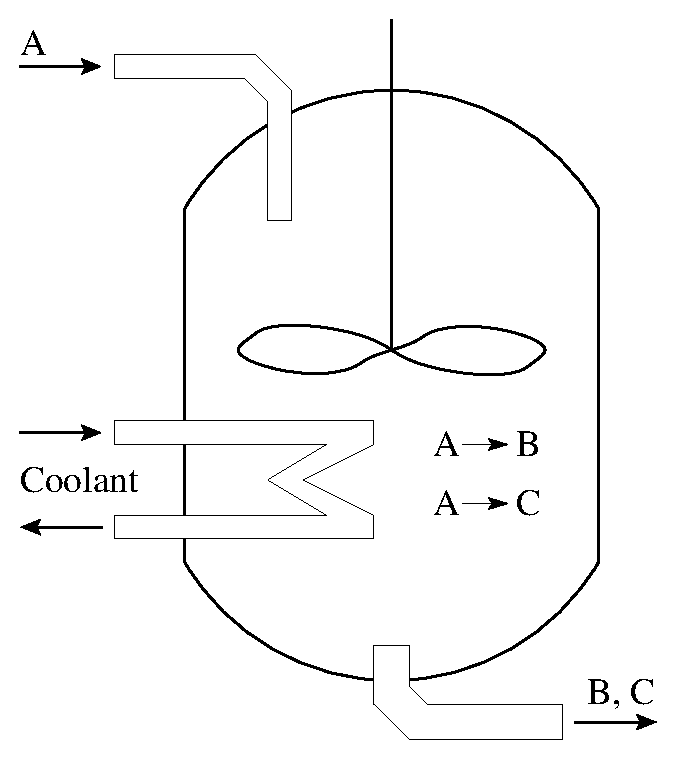
\includegraphics[width=0.4\textwidth,%
  totalheight=0.3\textheight]{cstr_picture}\\
\caption{Схема химического реактора.}%
\label{fig:cstr_picture}
\end{figure}


В работе~\cite{vas-bak2009} приводятся параметры объекта и ПИД
регулятора, а также проводится сравнение качества управления между
ПИД, нечетким и предлагаемым нейросетевым регулятором с ПИД входами.
В качестве критерия качества используется интегральная ошибка
управления на заданном сигнале уставки.  Пример ПИД управления для
ступенчато изменяющейся уставки приводится
на~\figref{fig:cstr_pid_ru}.

\begin{figure}[h]
\centering
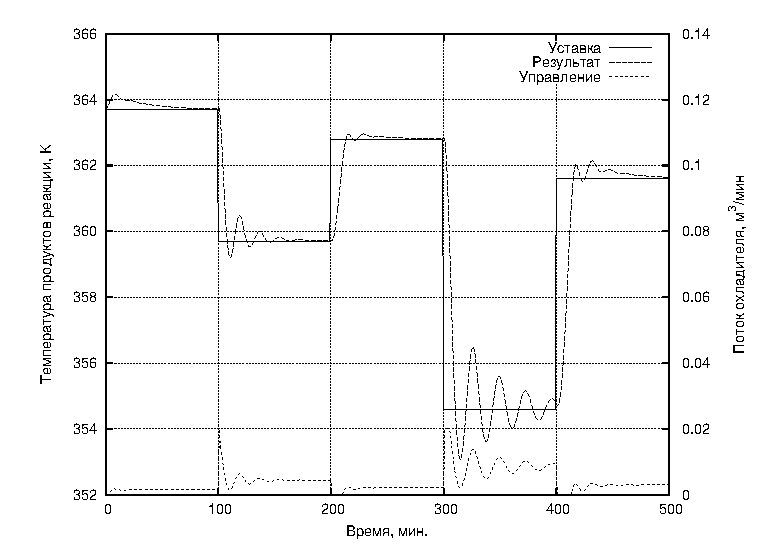
\includegraphics[width=0.8\textwidth,%
  totalheight=0.35\textheight]{cstr_pid_ru}
\caption{Пример управления реактором с помощью ПИД регулятора.}%
\label{fig:cstr_pid_ru}
\end{figure}

Типичный режим работы реактора --- обеспечение постоянного соотношения
продуктов $B$ и $C$ на выходе в течение достаточно длительного
времени.  В то же время, иногда требуется изменение этого соотношения.
Применяя полученные ранее рекомендации
(с.~\pageref{nnc-inputs-rules}), выбираем структуру входов
$r_k,e_k\ldots e_{k-d}$.  Объект управления достаточно инерционен,
поэтому возьмем $d=5$ чтобы НС--Р через память ошибки управления
обладал информацией о реакции объекта на предыдущие управляющие
воздействия.  Учитывая нелинейность объекта управления, возьмем сеть с
двумя скрытыми слоями: $\NN^p_{r_k+e_k+\ldots+e_{k-5},9,5}$.  Для
демонстрации важности наличия памяти ошибки управления на входе НС--Р,
возьмем для экспериментов также сеть архитектуры $\NN^p_{r_k+e_k,7,4}$
без памяти ($d=1$).

Обучение обеих сетей проводилось на одинаковых экспериментальных
выборках.  Графики ошибки в процессе обучения приведены
на~\figref{fig:cstr_e5r1_vs_e1r1_training}.  Видно, что обучение НС--Р
с архитектурой $\NN^p_{r_k+e_k,7,4}$ ($d=1$) закончилось досрочно в
силу начала роста ошибки на тестовой выборке, что свидетельствует о
потере сетью обобщающей способности.  В то же время, более сложная по
количеству нейронов сеть $\NN^p_{r_k+e_k+\ldots+e_{k-5},9,5}$ ($d=5$)
продолжает учиться, то есть, дополнительные входы
$e_{k-1},\ldots,e_{k-5}$ действительно несут полезную информацию для
обучения и могут эффективно использоваться сетью для обобщения.

\begin{figure}[h]
  \centering
  \begin{tabular}{cc}
    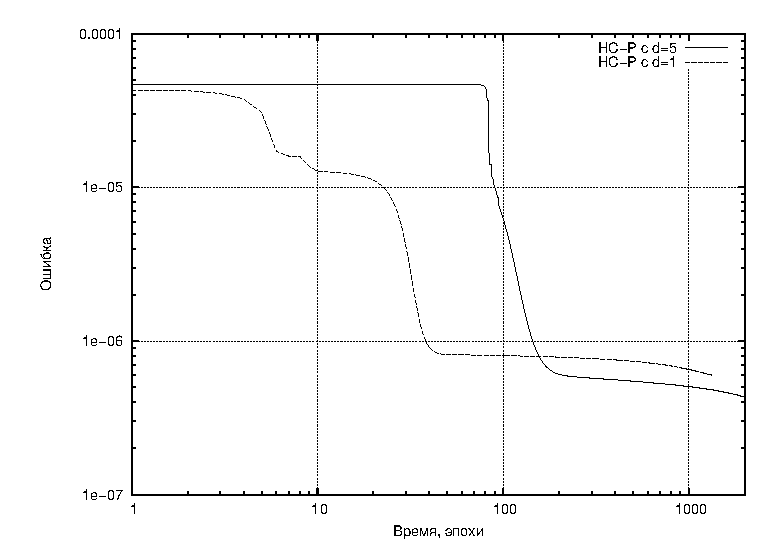
\includegraphics[width=0.45\textwidth,%
      totalheight=0.25\textheight]{cstr_e5r1_vs_e1r1_training_learn_rus}
    &
    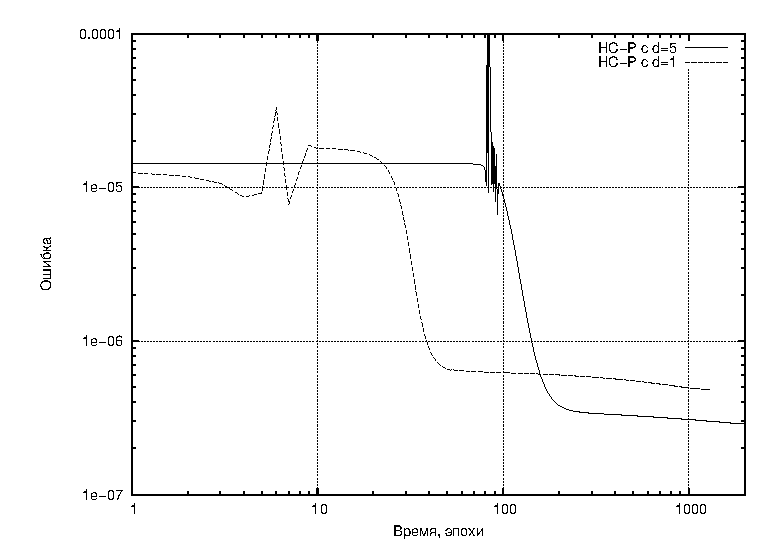
\includegraphics[width=0.45\textwidth,%
      totalheight=0.25\textheight]{cstr_e5r1_vs_e1r1_training_test_rus} \\
    а) & б)
  \end{tabular}
  \caption{Ошибка в процессе обучения НС--Р на обучающей (а) и тестовой (б) выборке.}%
  \label{fig:cstr_e5r1_vs_e1r1_training}
\end{figure}

Проверка нейронных сетей обеих архитектур вне контура управления не
выявляет качественного различия, хотя ошибка имитации сети
$\NN^p_{r_k+e_k+\ldots+e_{k-5},9,5}$ прогнозируемо несколько меньше,
чем у $\NN^p_{r_k+e_k,7,4}$ --- $2.89\times 10^{-7}$ против $4.85\times
10^{-7}$ (см. также~\figref{fig:cstr_pid_vs_nnc_contest_rus}а).  Однако в
контуре управления поведение нейросетевых регуляторов кардинально
различается~(\figref{fig:cstr_pid_vs_nnc_contest_rus}б): НС--Р с памятью
прошлых значений ошибки ведет себя качественно эквивалентно ПИД
регулятору, в то время как НС--Р регулятор с входами $r_k,e_k$ ведет
себя существенно иначе, чем ПИД.  Среднеквадратическая ошибка
управления НС--Р архитектуры $\NN^p_{r_k+e_k+\ldots+e_{k-5},9,5}$
равна 1.00, а НС--Р с архитектурой $\NN^p_{r_k+e_k,7,4}$ --- 1.09.

\begin{figure}[h]
  \centering
  \begin{tabular}{cc}
    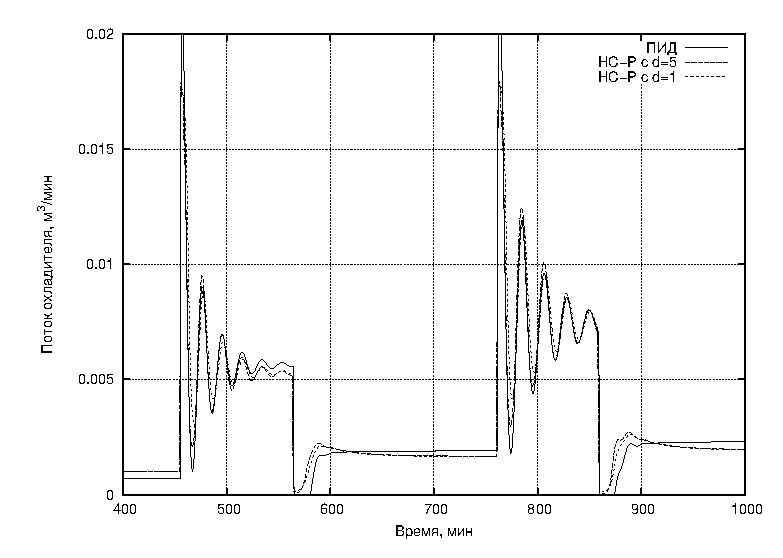
\includegraphics[width=0.45\textwidth,%
      totalheight=0.25\textheight]{cstr_e5r1_vs_e1r1_outloop_rus}
    &
    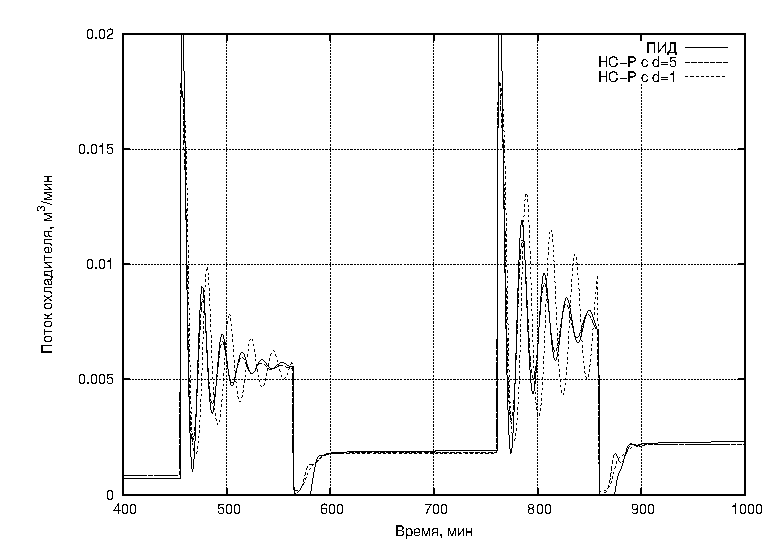
\includegraphics[width=0.45\textwidth,%
      totalheight=0.25\textheight]{cstr_e5r1_vs_e1r1_inloop_rus} \\
    а) & б) \\
  \end{tabular}
  \caption{Сравнение качества имитации НС--Р разных архитектур вне контура (а) и в контуре управления (б).}%
  \label{fig:cstr_pid_vs_nnc_contest_rus}
\end{figure}

Графики, позволяющие визуально оценить качество управления ПИД и его
нейросетевого имитатора с архитектурой
$\NN^p_{r_k+e_k+\ldots+e_{k-5},9,5}$ изображены
на~\figref{fig:cstr_pid_vs_nnc_inloop_rus}.  На данной выборке
среднеквадратическая ошибка управления для ПИД регулятора составила
$1.46$, а для НС--Р --- $1.31$.

\begin{figure}[h]
  \centering
  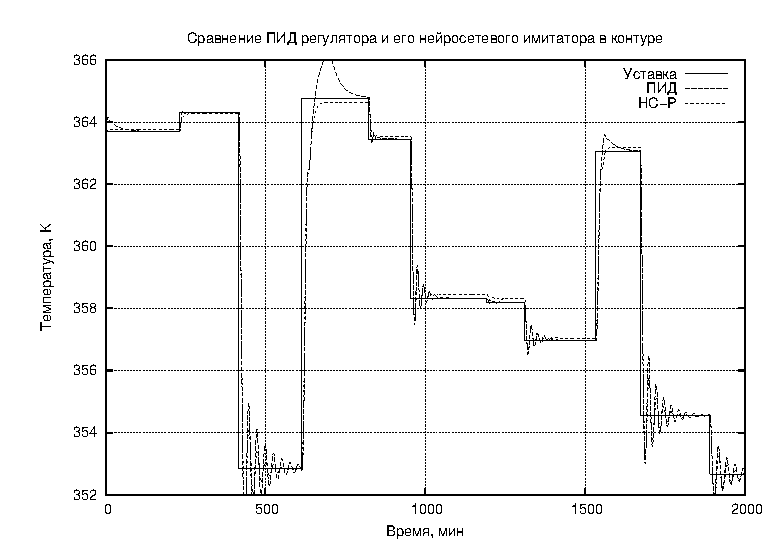
\includegraphics[width=0.8\textwidth,%
    totalheight=0.35\textheight]{cstr_pid_vs_nnc_inloop_rus} \\
  \caption{Сравнение ПИД и НС--Р в контуре управления.}%
  \label{fig:cstr_pid_vs_nnc_inloop_rus}
\end{figure}

Важно отметить, что по сравнению с ПИД регулятором, нейросетевой не
обеспечивает нулевую ошибку при постоянной уставке.  Это является
следствием статического характера функции нейронной сети и мерой
неточности полученного имитатора исходного регулятора.  Однако, данный
недостаток будет менее заметным при наличии помехи.

Переходный процесс при отработке понижения температуры для НС--Р
практически совпадает с ПИД, а повышение температуры уставки НС--Р
отрабатывает без заметного перерегулирования в отличие от ПИД.  Таким
образом, имеет место некоторое улучшение качества управления при
переходе от ПИД к НС--Р.  Это достаточно неожиданный результат, так
как задача улучшить качество управления не ставилась.
Предположительно эффект повышения качества при использовании НС--Р
связан со статической архитектурой сети, что исключает влияние
динамики регулятора на объект управления в отличие от ПИД, имеющего
собственные динамические характеристики.


\section{Выводы}

\begin{itemize}

\item Разработана методика по замене линейного регулятора на примере
  ПИД на нейросетевой.  Она может также применяться и для других видов
  регуляторов, так как предположение линейности исходного регулятора
  нигде не используется явно.

\item Исследован вопрос выбора набора входов для нейросетевого
  регулятора.  Для случая переменной уставки предложено использование
  входов $r_k,e_k\ldots e_{k-d}$, представляющее собой комбинированный
  подход к управлению по возмущению и отклонению.  Для задачи
  стабилизации (постоянная уставка) предложено использование входов
  $e_k\ldots e_{k-d}$.  Данные рекомендации обоснованы результатами
  вычислительных экспериментов.

\item Для имитации ПИД регулятора обосновано применение простых
  двухслойных персептронов с нелинейными нейронами.

\item Предложен метод рационального формирования обучающей выборки.
  Для её получения исследованы разные типы пробных сигналов и выявлен
  оптимальный с точки зрения качества нейросетевой апроксимации ---
  стохастический.

\item На примере показано успешное применение методики по замене ПИД
  регулятора на нейросетевой в системе управления с нелинейным
  объектом.

%TODO
%\item Если будет систематическое сравнение регуляторов, то тут добавить


\end{itemize}
